\textbf{J}
\begin{figure}[H]
  \centering
  \begin{subfigure}{0.1\textwidth}
    \centering
    \begin{tikzpicture}[scale=0.8]
      \draw(0,0) -- (0,0);
    \end{tikzpicture}
  \end{subfigure}
  \begin{subfigure}{.4\textwidth}
    \centering
    \begin{Karnaugh}{Y}{Z}{ZERO}{SP'}
      \minterms{7}
      \indeterminats{8, 9, 10, 11, 12, 13, 14, 15}
      \implicant[3pt]{7}{15}{blue}
    \end{Karnaugh}
  \end{subfigure}
  \begin{subfigure}{.4\textwidth}
    \centering
    \begin{Karnaugh}{Y}{Z}{ZERO}{SP'}
      \minterms{6, 7}
      \indeterminats{8, 9, 10, 11, 12, 13, 14, 15}
      \implicant[3pt]{7}{15}{blue}
      \implicant{7}{14}{red}
    \end{Karnaugh}
  \end{subfigure}

  \begin{subfigure}{0.5\textwidth}
    \centering
    \begin{tikzpicture}[scale=0.8]
      \draw(0,0) -- (0,0);
    \end{tikzpicture}
  \end{subfigure}
  \begin{subfigure}{.4\textwidth}
    \centering
    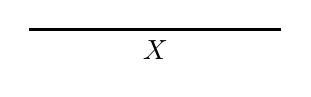
\begin{tikzpicture}[scale=0.8]
      \draw[very thick] (0,0.3) -- node [below]{$X$} ++(4,0);
    \end{tikzpicture}
  \end{subfigure}
  \caption*{$J_Y = \color{blue} \text{Z} \cdot \text{ZERO} \cdot \text{SP'} \color{black} + \color{red} \text{X} \cdot \text{Z} \cdot \text{ZERO} $.}
\end{figure}

\textbf{K}
\begin{figure}[H]
  \centering
  \begin{subfigure}{0.1\textwidth}
    \centering
    \begin{tikzpicture}[scale=0.8]
      \draw(0,0) -- (0,0);
    \end{tikzpicture}
  \end{subfigure}
  \begin{subfigure}{.4\textwidth}
    \centering
    \begin{Karnaugh}{Y}{Z}{ZERO}{SP'}
      \minterms{14, 15}
      \indeterminats{0, 1, 2, 3, 4, 5, 6, 7}
      \implicant{7}{14}{blue}
    \end{Karnaugh}
  \end{subfigure}
  \begin{subfigure}{.4\textwidth}
    \centering
    \begin{Karnaugh}{Y}{Z}{ZERO}{SP'}
      \minterms{14, 15}
      \indeterminats{0, 1, 2, 3, 4, 5, 6, 7}
      \implicant{7}{14}{blue}
    \end{Karnaugh}
  \end{subfigure}

  \begin{subfigure}{0.5\textwidth}
    \centering
    \begin{tikzpicture}[scale=0.8]
      \draw(0,0) -- (0,0);
    \end{tikzpicture}
  \end{subfigure}
  \begin{subfigure}{.4\textwidth}
    \centering
    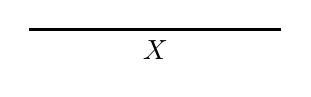
\begin{tikzpicture}[scale=0.8]
      \draw[very thick] (0,0.3) -- node [below]{$X$} ++(4,0);
    \end{tikzpicture}
  \end{subfigure}

  \caption*{$K_Y = \color{blue} \text{Z} \cdot \text{ZERO}$.}
\end{figure}
